\chapter{Practical aspects of DFT}
\label{sec:Practical DFT}

\section{The Exchange-Correlation functional}
From the topics covered in chapter 4 we know that the missing piece of the density functional theory is the complex exchange-correlation energy $E_{\text{xc}}[n]$, that must account for all the simplifications and approximations employed in Kohn-Sham DFT. In this section we will explore some of the most commonly used approximations to the exchange-correlation functional. Specifically we will look at 4 levels of complexity: first is the local density approximation (LDA), followed by the generalized gradient approximation (GGA). These two are the least complex and most computationally affordable methods. Next are meta-GGA and finally the very accurate, but equally demanding hybrid-functionals. In addition, we have methods such as DFT+U, the Minnesota functionals, double hybrids and more, but these are outside the scope of this project. The different methods mentioned above with increasing level of complexity and accuracy are often referred to as steps in Jacob's ladder, developed by Perdew \cite{jacob}. The ladder is illustrated below in figure 5.1. 

\begin{figure}[H]
\centering
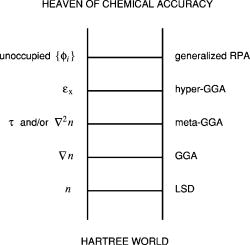
\includegraphics[width=.5\textwidth]{method/dft/jacob.jpeg}
\caption{Jacob's ladder \cite{jacob}.}
\end{figure}

   

\subsection{Local density approximation}
A homogeneous electron gas (HEG) is the sole case we know of where the exchange-correlation functional can be determined exactly, because in this simple case the electron density is constant. The LDA works by setting the exchange-correlation potential $V_\text{XC}(\boldsymbol{r})$ at every position equal to that of the homogeneous electron gas, ie

\begin{equation}
V_\text{XC}(\boldsymbol{r}) = V_\text{XC} ^\text{HEG}[n(\boldsymbol{r})] .
\end{equation} 

Obviously the LDA is of limited use given that a large part of what makes materials interesting is the variation in the electronic density. In the case of limitations LDA is for example known to overestimate binding energies and  underestimate the band gap in semiconductors and insulators. On the other hand, LDA provides generally adequate results in bulk materials with slowly varying charge density, for example equilibrium distances and vibrational frequencies. The biggest upside of LDA however comes from the low computational cost, and was one of the first big success-stories of DFT. 


\subsection{Generalized gradient approximation}
A natural succession to the local density approximation is the family of generalized gradient approximation (GGA) that also includes the gradient of the electron density

\begin{equation}
V_\text{XC} ^\text{GGA} (\boldsymbol{r}) = V_\text{XC} [n(\boldsymbol{r}), \nabla n(\boldsymbol{r})].
\end{equation}

The ways one can implement the gradient are plenty-full and complicated. Two of the most common methods are the Perdew-Wang 91 (PW91) \cite{pw91} and the Perdew-Burke-Ernzerhof (PBE) GGA \cite{pbe}. This project will utilize the latter, which came to fruition in  1996 in an article by Perdew, Burke and Ernzerhof appropriately named "Generalized Gradient Approximation Made Simple". The key point regarding the PBE functional is that it's a non-empirical method thus providing reliable and adequate accuracy over a wide range of systems, as compared to for instance the BLYP functional that provides excellent accuracy of organic molecules but fails in other cases \cite{PBE_forum}. 

\subsection{Meta-GGA}   
Meta-GGA functionals are the final level of complexity of the non-empirical approximations to the exchange-correlation functional. In addition to the constant density (LDA) and local gradient of the density (GGA), meta-GGA methods consider the kinetic energy density of the occupied Kohn-Sham orbitals \cite{metagga}
 
\begin{equation}
	\tau_\omega = \sum_i ^\text{occ}\frac{1}{2}|\nabla_{\psi_{i, \omega}}|^2.
\end{equation}

The importance of this quantity on the band gap is well described in \cite{xc_kineticEnergy}. In this project we employ a meta-GGA functional named \textit{Strongly Constrained Appropriately Normed}, or SCAN. This functional is the only known functional to satisfy all 17 known exact constraints of the XC functional \cite{scan}. The SCAN functional has found to provide superior accuracy of energies and geometries, especially in diversely bonded structures \cite{scan_divbond}, there is some indication of improved band gaps and density of states over GGA and LDA functionals \cite{scan_pbe}. However, it delivers overall less accurate band gaps compared to other meta-GGA functionals such as the \textit{modified Becke-Johnson} \cite{mbj}. Unfortunately, MBJ proved too difficult to converge for the particular materials in this project and we instead opt for SCAN. 
\begin{figure}[H]
\centering
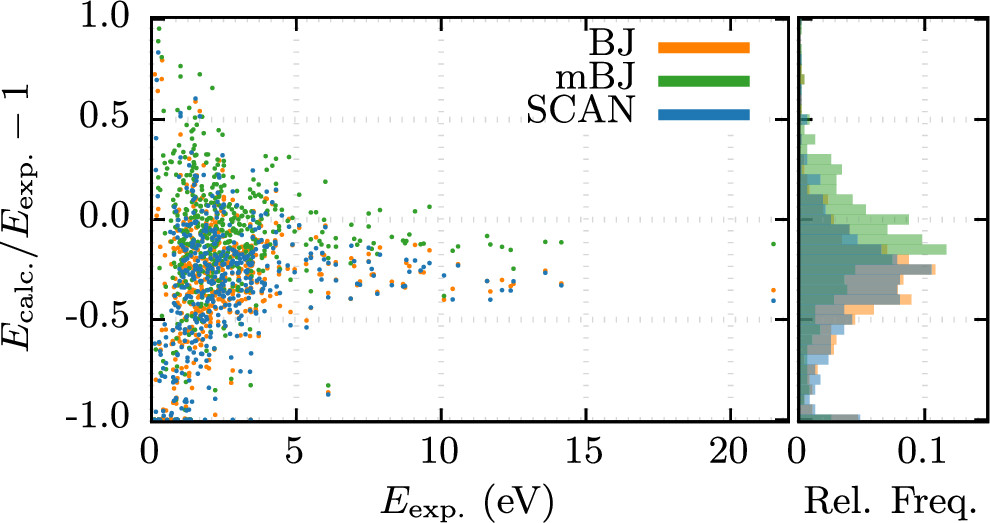
\includegraphics[scale=0.3]{method/dft/metagga.jpeg}
\caption{Calculated to experimental band gap measurements of Becke-Johnsoon, modified Becke-Johnson and SCAN functionals \cite{xc_benchmark}}
\end{figure}

\subsection{Hybrid functionals}

The most accurate functional we employ in this project belongs to the family of \textit{hybrid functionals}. This method consists of a hybrid between simpler functionals such as LDA, PBE or even meta-GGA and the exact treatment of exchange energy from Hartree-Fock, for example the global hybrid functional PBE0 \cite{pbe0} described as

\begin{equation}
E_\text{xc} ^\text{PBE0} = (1-\alpha)E_x ^\text{PBE} + \alpha E_x ^{HF} + E_c ^{PBE}, 
\end{equation}

 where $\alpha$ is the mixing parameter to decide the balance between the exchange energy, denoted $x$ of Hartree-Fock with PBE. Similarly the last term represents the correlation energy from the PBE functional. This parameter $\alpha$ is determined empirically, thus this is a semi-empirical model. Heyd-Scuseria-Ernzerhof improved the accuracy of the model by separating the Coulomb interaction into long-range and short-range interaction by a function erfc($\mu r$). These are known as HSE functionals \cite{hse}, one of the superior methods for accurate band gaps is the HSE06 hybrid functional \cite{hse06}, with $\alpha = 0.25$ and $\mu = 0.11$.  
 
\subsection{Outlook} 
 
In many cases LDA and GGA suffice, PBE especially is by most considered the conventional standard for DFT calculations, for its balance of accuracy, cost and wide range applicability. However, distinctly concerning the band gap of a solid, both of these fall short. This is because the band gap of DFT calculations is complicated by the fact that the derivative of the XC-functional is discontinuous with respect to the electron concentration \cite{xc_derivative}. Thus, the simpler functionals fail to recall the experimental values since the total band gap in DFT is the fundamental gap (valence - conduction) + this contribution. This is corrected in meta-GGA and hybrid functionals in the generalized Kohn-Sham scheme. Lastly, we would like to refer the reader to the work of Borlido et al. who in 2019 conducted an exhaustive investigation of the band gap of over 470 unique non-magnetic compounds in order to benchmark the relative performance of several of the available and widely used XC-functionals \cite{xc_benchmark}. In this large-scale project they found overwhelming confirmation that the HSE06 functional followed closely by Modified-Becke Johnson is the superior choice for accurate band-gap measures. Regarding the SCAN functional, in several cases this yielded outputs very comparable to MBJ, and produces much better formation energies than PBE, but tend to overestimate in magnetic alloys. On the other side, both LDA and PBE resulted in $50\%$ and $30\%$ under-estimation of the band gap or in several cases miss-classified compounds as metals. This was particularly evident in materials containing Ni and other 3d elements.  
 

\section{Plane waves and reciprocal space}
In this section, we will cover some of the practical factors that are important to consider when performing DFT calculations. The two most central topics are the energy cutoff parameter of plane waves, and the number of points in reciprocal space. More details on these parameters and relevant examples can be read about in \cite{Sholl2009}. 
 
The Shr\"{o}dinger equation for a free electron has a simple analytic solution $\psi_k = Ae^{i\boldsymbol{k}\boldsymbol{r}}$. In a crystalline matter with a periodic potential $V(\boldsymbol{r}) = V(\boldsymbol{r} + \boldsymbol{R})$, the single-electron wavefunction takes the form 

\begin{equation}
\psi_{\boldsymbol{k}}(\boldsymbol{r}) = u_{\boldsymbol{k}}(\boldsymbol{r})e^{i\boldsymbol{k}\boldsymbol{r}},    
\end{equation}

where $u_{\boldsymbol{k}}(\boldsymbol{r})$ is a Bloch wave with the periodicity of the crystal and $e^{ikr}$ is called a plane wave. Because DFT apply plane waves as basis functions of the electronic density, DFT calculations are often referred to as plane wave calculations. The Bloch wave is the sum of all plane waves with wave vector equal to the reciprocal wave vector $\boldsymbol{G}$, described as 

\begin{equation}
    u_{\boldsymbol{k}}(\boldsymbol{r}) = \sum_{\boldsymbol{G}} c_{\boldsymbol{G}}e^{i\boldsymbol{G}\boldsymbol{r}},
\end{equation}
 which gives us the final expression for $\psi_k (\boldsymbol{r})$ 
 
\begin{equation}
    \psi_{\boldsymbol{k}}(\boldsymbol{r}) = \sum_{\boldsymbol{G}} c_{\boldsymbol{k} + \boldsymbol{G}}e^{i(\boldsymbol{k} + \boldsymbol{G})\boldsymbol{r}}
\end{equation}

Clearly, the infinite summation over all $\boldsymbol{G}$ required to evaluate the wavefunction at a single point in reciprocal space is computationally unfeasible. In order to reduce this computational burden, we can introduce a maximum cutoff value of the energy $E_{\text{cut}}$. This is possible because equation 5.7 is the solution of the Shr\"{o}dinger equation with corresponding kinetic energy 

\begin{equation}
    E = \frac{\hbar^2}{2m}|\boldsymbol{k} + \boldsymbol{G}|^2.
\end{equation}

Assuming that the lower energy plane waves can represent the density adequately, we can limit the calculations to plane waves with energy less than $E_{\text{cut}}$:
\begin{equation}
    E_{\text{cut}} = \frac{\hbar^2}{2m}G_{\text{cut}}.
\end{equation}

Thus, we can reduce the infinitely large sum above to a much more feasible calculation
\begin{equation}
    \psi_{\boldsymbol{k}}(\boldsymbol{r}) = \sum_{|\boldsymbol{k} + \boldsymbol{G}| < G_{\text{cut}}} u_{\boldsymbol{k} + \boldsymbol{G}}(\boldsymbol{r})e^{i(\boldsymbol{k} + \boldsymbol{G})\boldsymbol{r}}.
\end{equation}

The cutoff energy can be determined by performing a number of calculations with different cutoffs and observe the convergence with respect to the total energy and other relevant properties of the system. Another important parameter to specify in DFT calculations is the number of k-points. As seen in the above expression the wavevector $k$ plays a big role in DFT. An other case that is more convinient to calculate in k-space is integrals of the form 
\begin{equation}
    g = \frac{V_{\text{cell}}}{(2\pi)^3} \int_{\text{BZ}} g(\boldsymbol{k})d\boldsymbol{k},
\end{equation}
for instance the density of states. Note that "BZ" indicates that the integral is evaluated for all $\boldsymbol{k}$ in the Brillouin zone. This integral can be approximated by evaluating it at a set of discrete k-points in reciprocal space and summing over the points with appropriately assigned weights. A larger set of points leads to more exact approximations. The method for selecting k-points in reciprocal space was developed by Monkhorst and Pack in 1976, where one specifies a number of points in each dimension $N_1 x N_2 x N_2$. Recalling that reciprocal space is inverse to regular space, supercells with equal and large dimensions converge at smaller values of $N$, and inversely for cells of small dimension. The total number of k-points required for converged calculations can be reduced by utilizing the symmetry of the cell, in which we can exactly approximate the entire BZ by extending a lesser zone through symmetry of the crystal lattice. This reduced zone is named the irreducible Brillouin zone (IBZ). 

The required number of k-points for a given calculation can be found alike the cutoff energy by performing convergence tests with respect to the total energy of the system. Metals in particular require a large number of k-points because of discontinues integrals in the Brillouin zone around the Fermi surface where the states discontinuously change from occupied to non-occupied. To reduce the cost of this operation, there are two primary methods: efficient sampling with the tetrahedron method, and smearing. The idea behind the tetrahedron method is to use a discrete set of k-points to fill the reciprocal space with tetrahedra and interpolate the function within each tetrahedron such that the function can be integrated in the entire space rather than at discrete points. The latter approach for solving discontinuous integrals is to smear out the discontinuity at the Fermi level and thus transforming the integral to a continuous one. A good analogy to this method is the Fermi-Dirac function, in which a small variable $\sigma$ transforms a step-function into a continuous function that can be integrated by standard methods.

A final consideration to how DFT is applied in practice is how the core electrons are handled. Tightly bound core electrons as opposed to valence electrons, demand a greater number of plane-waves to converge. The most efficient method of reducing the expenses of core-electrons are so-called pseudopotentials. This method works by approximating the electron density of the core electrons by a fixed density that mimics the properties of true ion core and core electrons. This density is then fixed for all subsequent calculations, in other words only considering the valence electrons while regarding the core electrons as frozen in. Two very popular pseudopotentials used in DFT are currently so-called ultrasoft psudopotentials (USPPs) developed by Vanderbilt, and the projector augmented-wave (PAW) method by Bl\"{o}chl \cite{PAW1}, \cite{PAW2}.

\section{Self-consistent field calculation}

\begin{figure}[H]
\centering
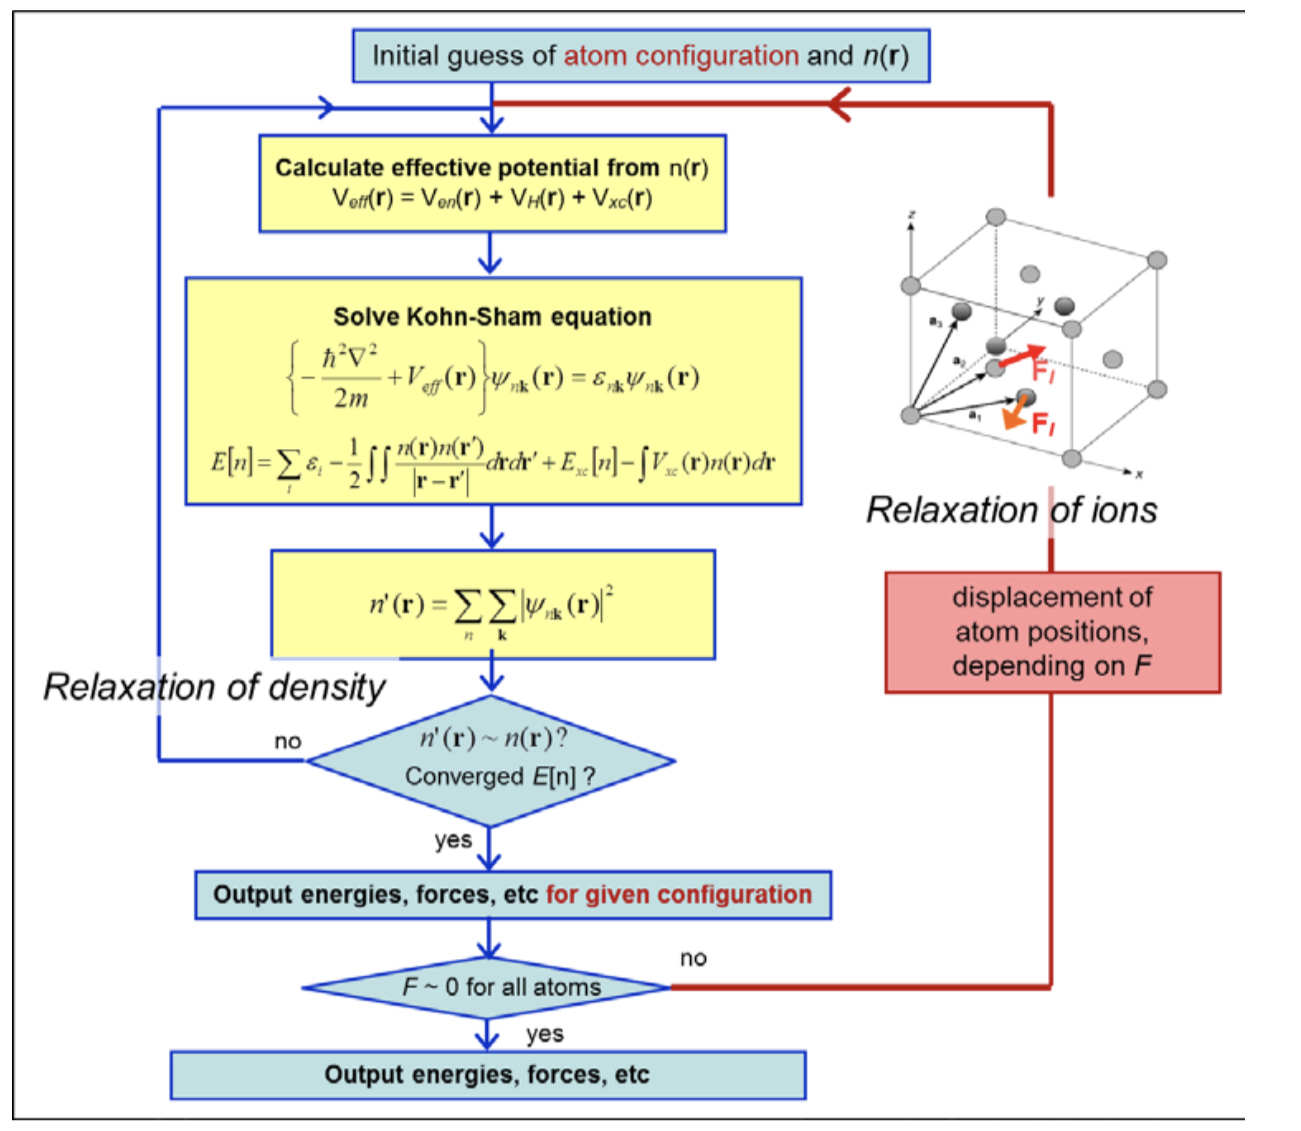
\includegraphics[width=\textwidth]{theory/selfConsistentDFT.jpeg}
\caption{Self consistent iterations of a DFT calculation. Figure adopted from the lecture notes in FYS-MENA4111 \cite{persson2020}}
\end{figure}

Preluding this section, we have considered the fundamental theory of DFT and its practical ability to model various materials. Figure 5.2 illustrates the self-consistent field calculation scheme for how DFT calculations are performed in practice. The initial problem posed by DFT is that all properties rely on the density, and are thus dependent on each other. For instance, the effective potential is dependent on the density, which again is dependent on the eigenfunctions, that rely on the effective potential again. The cleaver approach begins with an initial guess to the density from which we can solve the Kohn-Sham equations and obtain the corresponding eigenfunctions. Following is an iterative method where we apply the recently calculated eigenfunctions to determine a new density and repeat the procedure above. This is repeated until the total energy is converged, by an own-defined criterion. Equivalently, the optimal ionic positions can be found by a similar approach. This method is based on quasi-Newton algorithms to minimize the forces between ions. 



